% Options for packages loaded elsewhere
\PassOptionsToPackage{unicode}{hyperref}
\PassOptionsToPackage{hyphens}{url}
%
\documentclass[
]{article}
\usepackage{amsmath,amssymb}
\usepackage{lmodern}
\usepackage{iftex}
\ifPDFTeX
  \usepackage[T1]{fontenc}
  \usepackage[utf8]{inputenc}
  \usepackage{textcomp} % provide euro and other symbols
\else % if luatex or xetex
  \usepackage{unicode-math}
  \defaultfontfeatures{Scale=MatchLowercase}
  \defaultfontfeatures[\rmfamily]{Ligatures=TeX,Scale=1}
\fi
% Use upquote if available, for straight quotes in verbatim environments
\IfFileExists{upquote.sty}{\usepackage{upquote}}{}
\IfFileExists{microtype.sty}{% use microtype if available
  \usepackage[]{microtype}
  \UseMicrotypeSet[protrusion]{basicmath} % disable protrusion for tt fonts
}{}
\makeatletter
\@ifundefined{KOMAClassName}{% if non-KOMA class
  \IfFileExists{parskip.sty}{%
    \usepackage{parskip}
  }{% else
    \setlength{\parindent}{0pt}
    \setlength{\parskip}{6pt plus 2pt minus 1pt}}
}{% if KOMA class
  \KOMAoptions{parskip=half}}
\makeatother
\usepackage{xcolor}
\usepackage[margin=1in]{geometry}
\usepackage{color}
\usepackage{fancyvrb}
\newcommand{\VerbBar}{|}
\newcommand{\VERB}{\Verb[commandchars=\\\{\}]}
\DefineVerbatimEnvironment{Highlighting}{Verbatim}{commandchars=\\\{\}}
% Add ',fontsize=\small' for more characters per line
\usepackage{framed}
\definecolor{shadecolor}{RGB}{248,248,248}
\newenvironment{Shaded}{\begin{snugshade}}{\end{snugshade}}
\newcommand{\AlertTok}[1]{\textcolor[rgb]{0.94,0.16,0.16}{#1}}
\newcommand{\AnnotationTok}[1]{\textcolor[rgb]{0.56,0.35,0.01}{\textbf{\textit{#1}}}}
\newcommand{\AttributeTok}[1]{\textcolor[rgb]{0.77,0.63,0.00}{#1}}
\newcommand{\BaseNTok}[1]{\textcolor[rgb]{0.00,0.00,0.81}{#1}}
\newcommand{\BuiltInTok}[1]{#1}
\newcommand{\CharTok}[1]{\textcolor[rgb]{0.31,0.60,0.02}{#1}}
\newcommand{\CommentTok}[1]{\textcolor[rgb]{0.56,0.35,0.01}{\textit{#1}}}
\newcommand{\CommentVarTok}[1]{\textcolor[rgb]{0.56,0.35,0.01}{\textbf{\textit{#1}}}}
\newcommand{\ConstantTok}[1]{\textcolor[rgb]{0.00,0.00,0.00}{#1}}
\newcommand{\ControlFlowTok}[1]{\textcolor[rgb]{0.13,0.29,0.53}{\textbf{#1}}}
\newcommand{\DataTypeTok}[1]{\textcolor[rgb]{0.13,0.29,0.53}{#1}}
\newcommand{\DecValTok}[1]{\textcolor[rgb]{0.00,0.00,0.81}{#1}}
\newcommand{\DocumentationTok}[1]{\textcolor[rgb]{0.56,0.35,0.01}{\textbf{\textit{#1}}}}
\newcommand{\ErrorTok}[1]{\textcolor[rgb]{0.64,0.00,0.00}{\textbf{#1}}}
\newcommand{\ExtensionTok}[1]{#1}
\newcommand{\FloatTok}[1]{\textcolor[rgb]{0.00,0.00,0.81}{#1}}
\newcommand{\FunctionTok}[1]{\textcolor[rgb]{0.00,0.00,0.00}{#1}}
\newcommand{\ImportTok}[1]{#1}
\newcommand{\InformationTok}[1]{\textcolor[rgb]{0.56,0.35,0.01}{\textbf{\textit{#1}}}}
\newcommand{\KeywordTok}[1]{\textcolor[rgb]{0.13,0.29,0.53}{\textbf{#1}}}
\newcommand{\NormalTok}[1]{#1}
\newcommand{\OperatorTok}[1]{\textcolor[rgb]{0.81,0.36,0.00}{\textbf{#1}}}
\newcommand{\OtherTok}[1]{\textcolor[rgb]{0.56,0.35,0.01}{#1}}
\newcommand{\PreprocessorTok}[1]{\textcolor[rgb]{0.56,0.35,0.01}{\textit{#1}}}
\newcommand{\RegionMarkerTok}[1]{#1}
\newcommand{\SpecialCharTok}[1]{\textcolor[rgb]{0.00,0.00,0.00}{#1}}
\newcommand{\SpecialStringTok}[1]{\textcolor[rgb]{0.31,0.60,0.02}{#1}}
\newcommand{\StringTok}[1]{\textcolor[rgb]{0.31,0.60,0.02}{#1}}
\newcommand{\VariableTok}[1]{\textcolor[rgb]{0.00,0.00,0.00}{#1}}
\newcommand{\VerbatimStringTok}[1]{\textcolor[rgb]{0.31,0.60,0.02}{#1}}
\newcommand{\WarningTok}[1]{\textcolor[rgb]{0.56,0.35,0.01}{\textbf{\textit{#1}}}}
\usepackage{graphicx}
\makeatletter
\def\maxwidth{\ifdim\Gin@nat@width>\linewidth\linewidth\else\Gin@nat@width\fi}
\def\maxheight{\ifdim\Gin@nat@height>\textheight\textheight\else\Gin@nat@height\fi}
\makeatother
% Scale images if necessary, so that they will not overflow the page
% margins by default, and it is still possible to overwrite the defaults
% using explicit options in \includegraphics[width, height, ...]{}
\setkeys{Gin}{width=\maxwidth,height=\maxheight,keepaspectratio}
% Set default figure placement to htbp
\makeatletter
\def\fps@figure{htbp}
\makeatother
\setlength{\emergencystretch}{3em} % prevent overfull lines
\providecommand{\tightlist}{%
  \setlength{\itemsep}{0pt}\setlength{\parskip}{0pt}}
\setcounter{secnumdepth}{-\maxdimen} % remove section numbering
\ifLuaTeX
  \usepackage{selnolig}  % disable illegal ligatures
\fi
\IfFileExists{bookmark.sty}{\usepackage{bookmark}}{\usepackage{hyperref}}
\IfFileExists{xurl.sty}{\usepackage{xurl}}{} % add URL line breaks if available
\urlstyle{same} % disable monospaced font for URLs
\hypersetup{
  pdftitle={nyc\_bikes\_presentation},
  pdfauthor={jane\_hogg},
  hidelinks,
  pdfcreator={LaTeX via pandoc}}

\title{nyc\_bikes\_presentation}
\author{jane\_hogg}
\date{2022-11-14}

\begin{document}
\maketitle

\begin{Shaded}
\begin{Highlighting}[]
\FunctionTok{library}\NormalTok{(tidyverse)}
\end{Highlighting}
\end{Shaded}

\begin{verbatim}
## -- Attaching packages --------------------------------------- tidyverse 1.3.2 --
## v ggplot2 3.3.6      v purrr   0.3.4 
## v tibble  3.1.8      v dplyr   1.0.10
## v tidyr   1.2.1      v stringr 1.4.1 
## v readr   2.1.3      v forcats 0.5.2 
## -- Conflicts ------------------------------------------ tidyverse_conflicts() --
## x dplyr::filter() masks stats::filter()
## x dplyr::lag()    masks stats::lag()
\end{verbatim}

\begin{Shaded}
\begin{Highlighting}[]
\FunctionTok{library}\NormalTok{(ggplot2)}
\FunctionTok{library}\NormalTok{(janitor)}
\end{Highlighting}
\end{Shaded}

\begin{verbatim}
## 
## Attaching package: 'janitor'
## 
## The following objects are masked from 'package:stats':
## 
##     chisq.test, fisher.test
\end{verbatim}

\begin{Shaded}
\begin{Highlighting}[]
\FunctionTok{library}\NormalTok{(ggplot2)}
\FunctionTok{library}\NormalTok{(lubridate)}
\end{Highlighting}
\end{Shaded}

\begin{verbatim}
## 
## Attaching package: 'lubridate'
## 
## The following objects are masked from 'package:base':
## 
##     date, intersect, setdiff, union
\end{verbatim}

\begin{Shaded}
\begin{Highlighting}[]
\FunctionTok{library}\NormalTok{(tsibbledata)}
\end{Highlighting}
\end{Shaded}

\begin{verbatim}
## Warning: package 'tsibbledata' was built under R version 4.2.2
\end{verbatim}

\begin{Shaded}
\begin{Highlighting}[]
\FunctionTok{library}\NormalTok{(dplyr)}
\end{Highlighting}
\end{Shaded}

\#\#\#Contents

Introduction Purpose of the Report summary of Findings - Top Take Aways
Deep Dive - Our Customers Trips Recommendations

\#\#\#Introduction

The data used is from Citi Bikes based in New York, New York. It is a
sample of 10 bikes useage in 2018. The start and stop time of use, start
geo-location, membership type, age and gender of the user is included in
the sample.

Citi Bikes was founded in May 2013 and is a bike sharing scheme, Bikes
are available 24/7 7 days a week all year round. There are well over
12,000+ bikes available across Manhattan, Brooklyn, Queens and Jersey
City and there was a total of 746 active bike locations by the end of
December 2018.

There are now a range of price points to access the scheme including
annual subscriptions, pay as you go and concessions. At the end of
December 2018 there were 3,653 annual members and 33,965 casual users
signed up or renewed. Total annual membership stood at 147,090 including
memberships purchased with Jersey City billing zip codes.

The data has been processed to remove trips that are taken by staff as
they service and inspect the system, trips that are taken to/from any
``test'' and any trips that were below 60 seconds in length (potentially
false starts or users trying to re-dock a bike to ensure it's secure).
There is no personal data included in the sample other than age/gender.

There are three points to note from the dataset that may lead us to
consider if the data is fully representative of the populations as a
whole. Firstly the sample is predominately male (72\% of the sample) and
as a consequence the results may be overly representative of them.
Secondly the sample is predominately monthly subscription members (xx of
the sample) and this data does not include any discounted, single-day
pass or single ride users.

Finally the bikes for rental are only suitable for fully-able bodied
individuals. There are no accessibility bikes or trikes and as a
consequence anyone with a disability or limited mobility would not have
been included in the data set as they could not access the bikes.

\#\#\#Purpose of the Report

There are two key questions below, but overall the aim of the work is to
provide insights and actions that could increase bike hire and revenues.

Do bike hire patterns differ between bike rider demographics?
(e.g.~gender, type of trip, age)

What is the pattern of bike hires over time (e.g.~within a year, month,
week, or day)?

\hypertarget{summary-of-findings}{%
\subsubsection{Summary of Findings}\label{summary-of-findings}}

Female users constitute only 21\% of the data set and there may be an
opportunity to attract more women to the service - Recommendation -
further research to consider if there are particular barriers to women
using the service or why we not attracting female users. Secondary data
is available to consider what theses barriers might be e.g confidence to
cycle, safety or a better understanding of women travel habits is
needed. In addition a change in the gender selections would be advisable
in the future to fully reflect options.

The age profile of the sample is predominately in the XX age bracket and
although the average age of a New Yorker is 37 there are still over 1.2m
people in New York over 65 - Recommendation - consider what the barriers
are to older people using the service; are the bikes suitable for older
people or people with additional needs?

Subscribers make up significant percentage of the sample - 92\%. Does
this pricing structure inhibit the more casual user taking more trips? -
Recommendation - undertake further research on the pricing strategy with
casual users or test alternative pricing strategies as part of
promotional work with target segments that are unlikely to undermine the
subscriber base e.g day/overnight visitors

July and August are the peak months for use - unsurprising considering
the weather and holiday season. But there is scope for growth in the
shoulder months Recommendation - there is an opportunity to grow the
autumn and spring months(when there is better weather) and increase
uptake of the service as the weather improves. The Christmas period,
lower uptake, but there still could be an opportunity to grow uptake if
the target is leisure.sightseeing users. e.g Elf/Santa Hunt !!

\#\#Our Customers -

\begin{Shaded}
\begin{Highlighting}[]
\NormalTok{tsibbledata}\SpecialCharTok{::}\NormalTok{nyc\_bikes}
\end{Highlighting}
\end{Shaded}

\begin{verbatim}
## # A tibble: 4,268 x 12
##    bike_id start_time          stop_time           start_station start~1 start~2
##    <fct>   <dttm>              <dttm>              <fct>           <dbl>   <dbl>
##  1 26301   2018-02-26 19:11:03 2018-02-26 19:15:40 3186             40.7   -74.0
##  2 26301   2018-02-27 07:52:49 2018-02-27 07:58:13 3203             40.7   -74.0
##  3 26301   2018-02-27 12:03:27 2018-02-27 12:04:54 3202             40.7   -74.0
##  4 26301   2018-02-27 13:53:51 2018-02-27 14:21:04 3638             40.7   -74.0
##  5 26301   2018-02-27 14:30:42 2018-02-27 14:33:11 3638             40.7   -74.0
##  6 26301   2018-02-27 16:31:04 2018-02-27 16:33:27 3187             40.7   -74.0
##  7 26301   2018-02-27 17:37:12 2018-02-27 17:40:49 3638             40.7   -74.0
##  8 26301   2018-02-27 17:49:10 2018-02-27 17:55:03 3639             40.7   -74.0
##  9 26301   2018-02-27 18:21:57 2018-02-27 18:25:18 3202             40.7   -74.0
## 10 26301   2018-02-27 22:08:55 2018-02-27 22:28:42 3638             40.7   -74.0
## # ... with 4,258 more rows, 6 more variables: end_station <fct>, end_lat <dbl>,
## #   end_long <dbl>, type <fct>, birth_year <dbl>, gender <fct>, and abbreviated
## #   variable names 1: start_lat, 2: start_long
\end{verbatim}

\begin{Shaded}
\begin{Highlighting}[]
\NormalTok{gender }\OtherTok{\textless{}{-}}\NormalTok{ nyc\_bikes }\SpecialCharTok{\%\textgreater{}\%} 
  \FunctionTok{select}\NormalTok{(gender)}\SpecialCharTok{\%\textgreater{}\%}
 \FunctionTok{count}\NormalTok{(gender)}

\NormalTok{gender}
\end{Highlighting}
\end{Shaded}

\begin{verbatim}
## # A tibble: 3 x 2
##   gender      n
##   <fct>   <int>
## 1 Unknown   269
## 2 Male     3069
## 3 Female    930
\end{verbatim}

\begin{Shaded}
\begin{Highlighting}[]
\FunctionTok{ggplot}\NormalTok{(gender)}\SpecialCharTok{+}
  \FunctionTok{geom\_bar}\NormalTok{(}\FunctionTok{aes}\NormalTok{(}\AttributeTok{x =}\NormalTok{ gender, }\AttributeTok{y =}\NormalTok{ n), }\AttributeTok{stat =} \StringTok{\textquotesingle{}identity\textquotesingle{}}\NormalTok{, }\AttributeTok{fill =} \StringTok{"lightblue"}\NormalTok{)}\SpecialCharTok{+}
 \FunctionTok{labs}\NormalTok{(}
    \AttributeTok{x =} \StringTok{"Gender"}\NormalTok{,}
    \AttributeTok{y =} \StringTok{"Number"}\NormalTok{,}
    \AttributeTok{title =} \StringTok{"Gender of Citibike Users"}\NormalTok{,}
    \AttributeTok{subtitle =} \StringTok{"2018 Data (Sample 4268)"}\NormalTok{,)}
\end{Highlighting}
\end{Shaded}

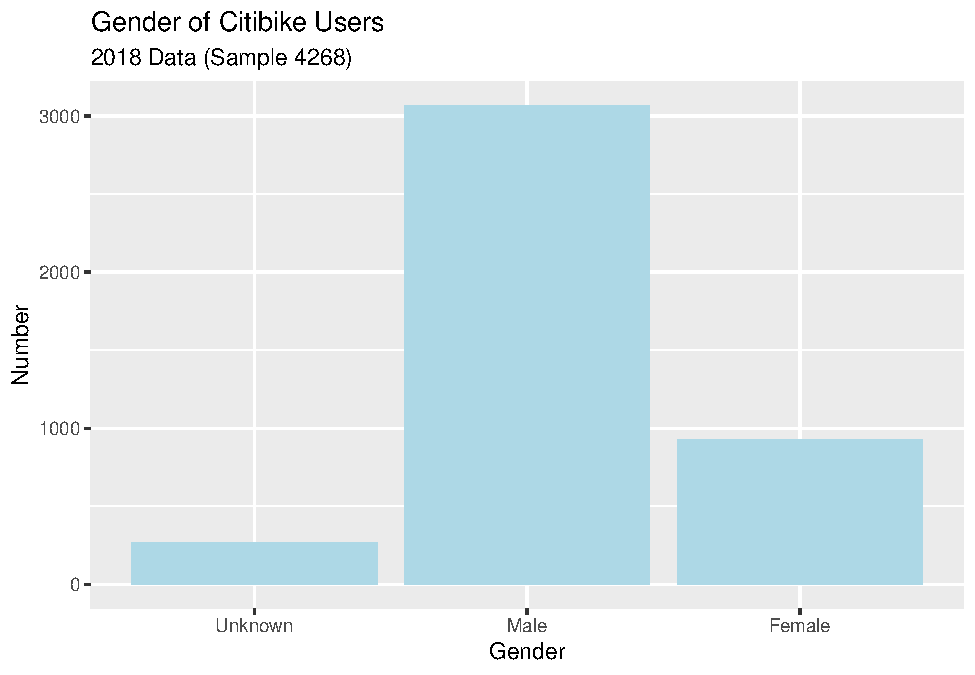
\includegraphics{nyc_bikes_presentation_janehogg_files/figure-latex/unnamed-chunk-4-1.pdf}

\#\#From the data we can see that there is a significantly higher number
of men in the survey results - 71\% of the sample with only 21\% female.
It should also be noted that 6\% of the sample did not respond to the
question.

\begin{Shaded}
\begin{Highlighting}[]
\NormalTok{sale\_type }\OtherTok{\textless{}{-}}\NormalTok{nyc\_bikes }\SpecialCharTok{\%\textgreater{}\%} 
  \FunctionTok{select}\NormalTok{(type)}\SpecialCharTok{\%\textgreater{}\%}
 \FunctionTok{count}\NormalTok{(type)}
\end{Highlighting}
\end{Shaded}

\begin{Shaded}
\begin{Highlighting}[]
\FunctionTok{ggplot}\NormalTok{(sale\_type)}\SpecialCharTok{+}
  \FunctionTok{geom\_bar}\NormalTok{(}\FunctionTok{aes}\NormalTok{(}\AttributeTok{x =}\NormalTok{ type, }\AttributeTok{y =}\NormalTok{ n), }\AttributeTok{stat =} \StringTok{\textquotesingle{}identity\textquotesingle{}}\NormalTok{, }\AttributeTok{fill =} \StringTok{"lightblue"}\NormalTok{)}\SpecialCharTok{+}
 \FunctionTok{labs}\NormalTok{(}
    \AttributeTok{x =} \StringTok{"Payment Method"}\NormalTok{,}
    \AttributeTok{y =} \StringTok{"Number"}\NormalTok{,}
    \AttributeTok{title =} \StringTok{"Payment Method of Citibike Users"}\NormalTok{,}
    \AttributeTok{subtitle =} \StringTok{"2018 Data (Sample 4268)"}\NormalTok{,)}
\end{Highlighting}
\end{Shaded}

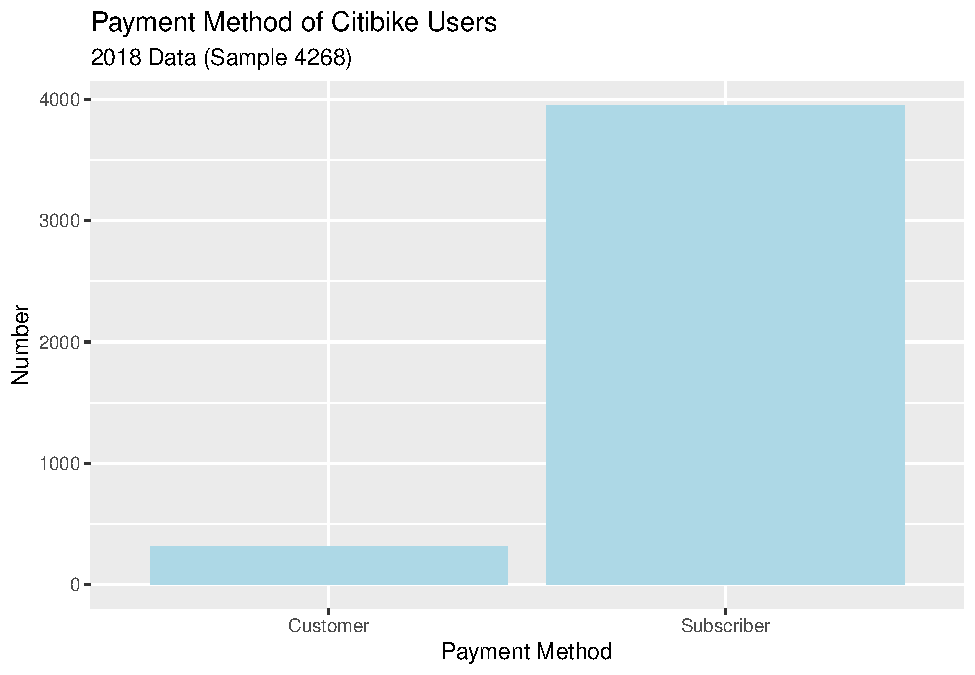
\includegraphics{nyc_bikes_presentation_janehogg_files/figure-latex/unnamed-chunk-6-1.pdf}

\#\#The majority of users were subscribers - 92\% of the sample with the
remaining 8\% being pay as you go. There are financial advantages of
securing a monthly payment over pay as you go fees, however this could
be limiting access to some segments of the market and there coud be
opportunities for growth, in particular for the tourist market or those
segments that are price sensitive.

\#\#Age profile of users

\begin{Shaded}
\begin{Highlighting}[]
\NormalTok{ age }\OtherTok{\textless{}{-}}\NormalTok{ nyc\_bikes}\SpecialCharTok{\%\textgreater{}\%}
  \FunctionTok{mutate}\NormalTok{(}\AttributeTok{age =} \DecValTok{2018} \SpecialCharTok{{-}}\NormalTok{ birth\_year)}
\end{Highlighting}
\end{Shaded}

\begin{Shaded}
\begin{Highlighting}[]
\FunctionTok{ggplot}\NormalTok{(age)}\SpecialCharTok{+}
  \FunctionTok{aes}\NormalTok{(}\AttributeTok{x =}\NormalTok{ age) }\SpecialCharTok{+}
  \FunctionTok{geom\_histogram}\NormalTok{(}\AttributeTok{bins =}\DecValTok{20}\NormalTok{, }\AttributeTok{colour =} \StringTok{"lightblue"}\NormalTok{)}\SpecialCharTok{+}
  \FunctionTok{labs}\NormalTok{(}
    \AttributeTok{x =} \StringTok{" Age "}\NormalTok{,}
    \AttributeTok{y =} \StringTok{"Number of Users"}\NormalTok{,}
    \AttributeTok{title =} \StringTok{"Age Profiles of Citibike Users"}\NormalTok{,}
    \AttributeTok{subtitle =} \StringTok{"2018 Data (Sample 4268)"}\NormalTok{,)}
\end{Highlighting}
\end{Shaded}

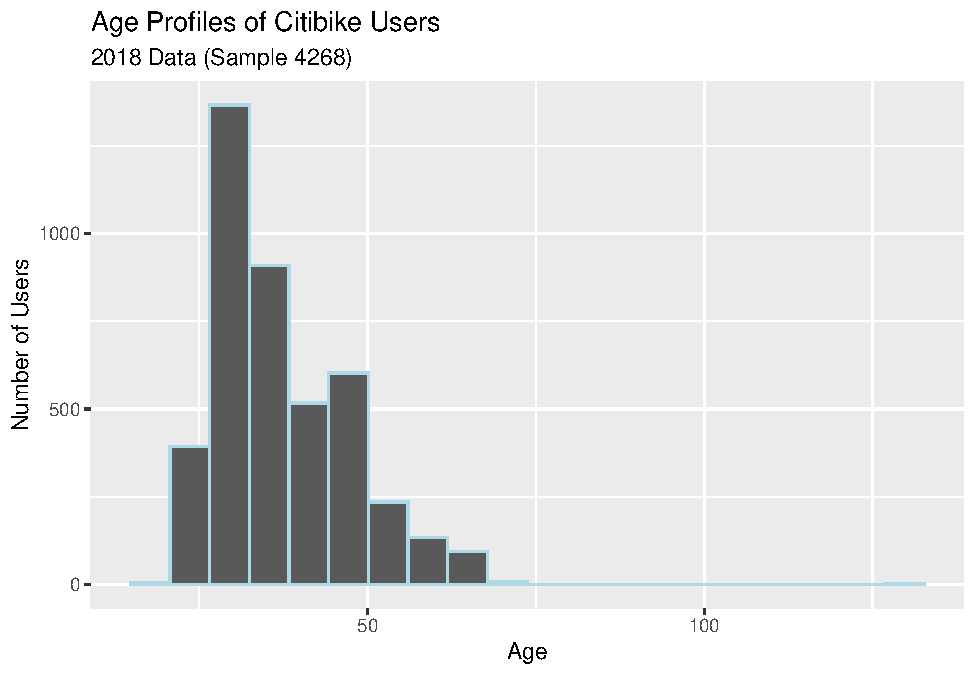
\includegraphics{nyc_bikes_presentation_janehogg_files/figure-latex/unnamed-chunk-8-1.pdf}

\begin{Shaded}
\begin{Highlighting}[]
\FunctionTok{ggplot}\NormalTok{(age)}\SpecialCharTok{+}
  \FunctionTok{aes}\NormalTok{(}\AttributeTok{x =}\NormalTok{ age) }\SpecialCharTok{+}
  \FunctionTok{geom\_histogram}\NormalTok{(}\AttributeTok{bins =}\DecValTok{10}\NormalTok{, }\AttributeTok{colour =} \StringTok{"lightblue"}\NormalTok{)}\SpecialCharTok{+}
  \FunctionTok{labs}\NormalTok{(}
    \AttributeTok{x =} \StringTok{" Age "}\NormalTok{,}
    \AttributeTok{y =} \StringTok{"Number of Users"}\NormalTok{,}
    \AttributeTok{title =} \StringTok{"Age Profiles of Citibike Users {-} Drill down"}\NormalTok{,}
    \AttributeTok{subtitle =} \StringTok{"2018 Data (Sample 4268)"}\NormalTok{,)}
\end{Highlighting}
\end{Shaded}

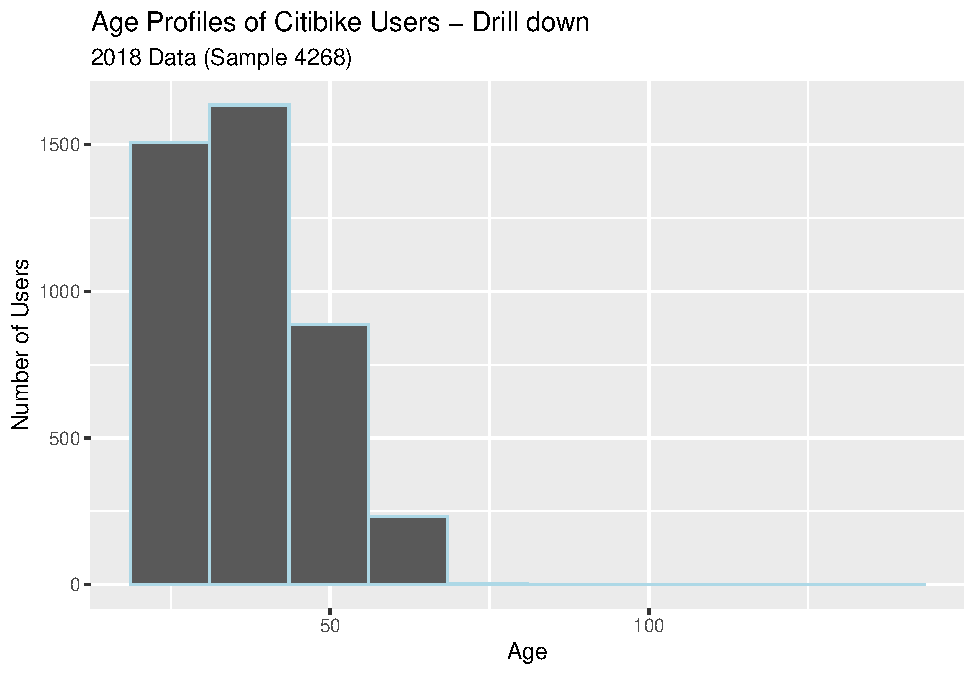
\includegraphics{nyc_bikes_presentation_janehogg_files/figure-latex/unnamed-chunk-9-1.pdf}

\hypertarget{the-age-profile-of-our-users-is-interesting-with-the-majority-being-under-55.}{%
\subsection{The age profile of our users is interesting with the
majority being under
55.}\label{the-age-profile-of-our-users-is-interesting-with-the-majority-being-under-55.}}

\#\#According to 2019 US population estimates 15.4\% of the total
population in New York are 65 years and over. There are currently
8.3million people in New York and this constitutes a potential market
size of 1,250,522. Not everyone in this age profile will be
willing/capable of cycle but targetting just 1\% of this market could
bring 12,505 new users. Recommend further research with the 55+ market
to consider demand and user needs.

\#\#\#Our Trips - Monthly Useage

\begin{Shaded}
\begin{Highlighting}[]
\NormalTok{nyc\_bikes\_df }\OtherTok{\textless{}{-}}\NormalTok{ nyc\_bikes }\SpecialCharTok{\%\textgreater{}\%}
  \FunctionTok{mutate}\NormalTok{(}\AttributeTok{day =} \FunctionTok{day}\NormalTok{(start\_time),}
         \AttributeTok{month =} \FunctionTok{month}\NormalTok{(start\_time),}\AttributeTok{label =} \ConstantTok{TRUE}\NormalTok{, }\AttributeTok{abbr =} \ConstantTok{FALSE}\NormalTok{,}
          \AttributeTok{year =} \FunctionTok{year}\NormalTok{(start\_time))}
\NormalTok{nyc\_bikes\_df }\OtherTok{\textless{}{-}}\NormalTok{ nyc\_bikes\_df }\SpecialCharTok{\%\textgreater{}\%}
  \FunctionTok{mutate}\NormalTok{(}\AttributeTok{age =}\NormalTok{ (year }\SpecialCharTok{{-}}\NormalTok{ birth\_year))}
\end{Highlighting}
\end{Shaded}

\begin{Shaded}
\begin{Highlighting}[]
\NormalTok{nyc\_bikes\_df }\SpecialCharTok{\%\textgreater{}\%}
  \FunctionTok{group\_by}\NormalTok{(month) }\SpecialCharTok{\%\textgreater{}\%}
  \FunctionTok{count}\NormalTok{() }\SpecialCharTok{\%\textgreater{}\%}
  \FunctionTok{summarise}\NormalTok{(n) }
\end{Highlighting}
\end{Shaded}

\begin{verbatim}
## # A tibble: 12 x 2
##    month     n
##    <dbl> <int>
##  1     1   132
##  2     2   112
##  3     3   173
##  4     4   326
##  5     5   459
##  6     6   498
##  7     7   637
##  8     8   728
##  9     9   432
## 10    10   416
## 11    11   213
## 12    12   142
\end{verbatim}

\begin{Shaded}
\begin{Highlighting}[]
\NormalTok{nyc\_bikes\_df }\SpecialCharTok{\%\textgreater{}\%}
  \FunctionTok{group\_by}\NormalTok{(month) }\SpecialCharTok{\%\textgreater{}\%}
  \FunctionTok{count}\NormalTok{() }\SpecialCharTok{\%\textgreater{}\%}
  \FunctionTok{summarise}\NormalTok{(n) }\SpecialCharTok{\%\textgreater{}\%}
\FunctionTok{ggplot}\NormalTok{(}\FunctionTok{aes}\NormalTok{(}\AttributeTok{x=}\NormalTok{ month, }\AttributeTok{y =}\NormalTok{ n))}\SpecialCharTok{+}
  \FunctionTok{geom\_point}\NormalTok{(}\AttributeTok{colour =} \StringTok{"blue"}\NormalTok{)}\SpecialCharTok{+}
  \FunctionTok{theme\_bw}\NormalTok{()}\SpecialCharTok{+}
  \FunctionTok{scale\_x\_continuous}\NormalTok{(}\AttributeTok{breaks =} \DecValTok{1}\SpecialCharTok{:}\DecValTok{12}\NormalTok{)}\SpecialCharTok{+}
  \FunctionTok{labs}\NormalTok{(}
    \AttributeTok{x =} \StringTok{" Months "}\NormalTok{,}
    \AttributeTok{y =} \StringTok{"Number of Users"}\NormalTok{,}
    \AttributeTok{title =} \StringTok{"Citibike Users each Month"}\NormalTok{,}
    \AttributeTok{subtitle =} \StringTok{"2018 Data (Sample 4268)"}\NormalTok{,)}
\end{Highlighting}
\end{Shaded}

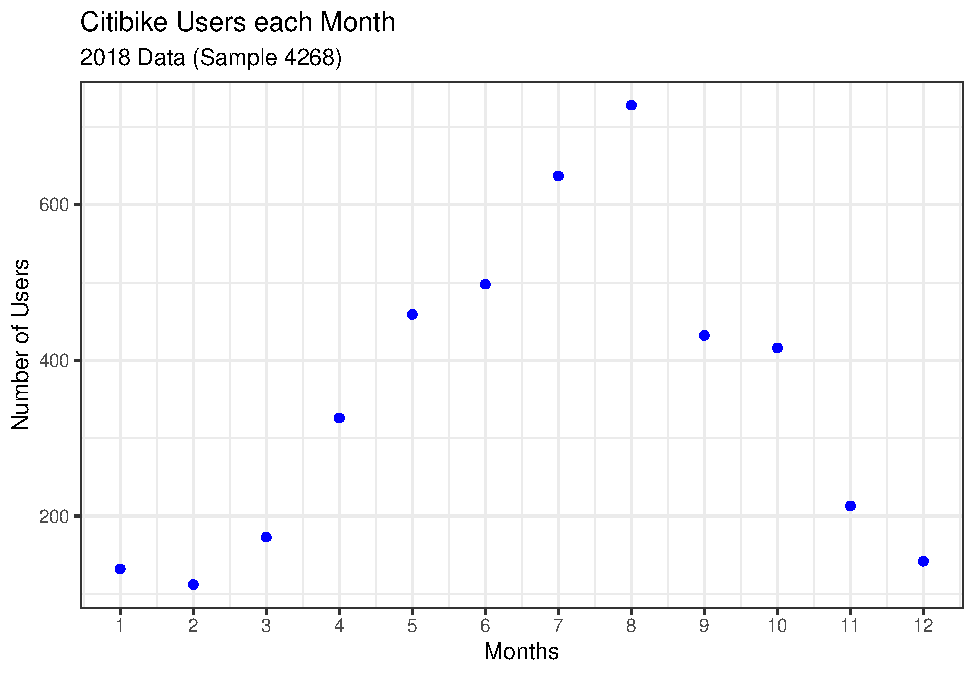
\includegraphics{nyc_bikes_presentation_janehogg_files/figure-latex/unnamed-chunk-12-1.pdf}

\#\#July and August are the most popular months corresponding to both
the driest months and the warmest. The lowest useage is in the spring
and the winter months were cyling requires extra clothing, care and also
there is more likely to be poor weather conditions e.g snow.

\#\#However there may still be opportunities to grow the useage during
periods where there are opportunities for tourists to enjoy
Christmas/New Year lights displays in the city.

\begin{Shaded}
\begin{Highlighting}[]
\NormalTok{nyc\_bikes\_df }\SpecialCharTok{\%\textgreater{}\%}
  \FunctionTok{group\_by}\NormalTok{(month, gender) }\SpecialCharTok{\%\textgreater{}\%}
  \FunctionTok{count}\NormalTok{() }\SpecialCharTok{\%\textgreater{}\%}
  \FunctionTok{summarise}\NormalTok{(n) }\SpecialCharTok{\%\textgreater{}\%}
\FunctionTok{ggplot}\NormalTok{(}\FunctionTok{aes}\NormalTok{(}\AttributeTok{x=}\NormalTok{ month, }\AttributeTok{y =}\NormalTok{ n, }\AttributeTok{group =}\NormalTok{ gender))}\SpecialCharTok{+}
  \FunctionTok{geom\_point}\NormalTok{(}\AttributeTok{colour =} \StringTok{"blue"}\NormalTok{)}\SpecialCharTok{+}
  \FunctionTok{theme\_bw}\NormalTok{()}\SpecialCharTok{+}
  \FunctionTok{scale\_x\_continuous}\NormalTok{(}\AttributeTok{breaks =} \DecValTok{1}\SpecialCharTok{:}\DecValTok{12}\NormalTok{)}\SpecialCharTok{+}
  \FunctionTok{facet\_wrap}\NormalTok{(}\SpecialCharTok{\textasciitilde{}}\NormalTok{gender)}\SpecialCharTok{+}
  \FunctionTok{labs}\NormalTok{(}
    \AttributeTok{x =} \StringTok{" Months "}\NormalTok{,}
    \AttributeTok{y =} \StringTok{"Number of Users"}\NormalTok{,}
    \AttributeTok{title =} \StringTok{"Variation in Use v Gender"}\NormalTok{,}
    \AttributeTok{subtitle =} \StringTok{"2018 Data (Sample 4268)"}\NormalTok{,)}
\end{Highlighting}
\end{Shaded}

\begin{verbatim}
## `summarise()` has grouped output by 'month'. You can override using the
## `.groups` argument.
\end{verbatim}

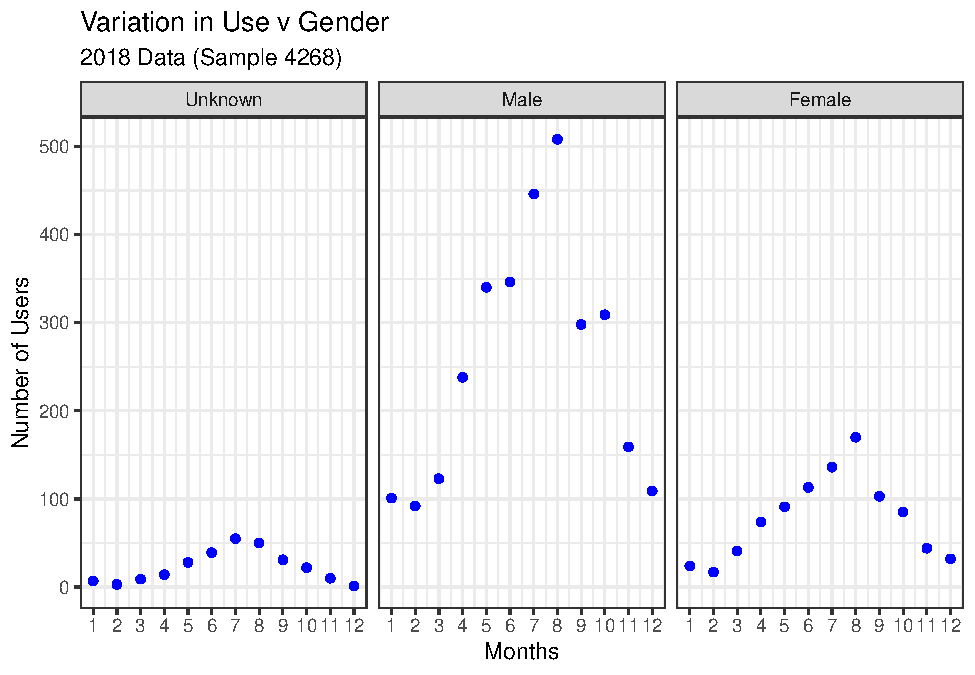
\includegraphics{nyc_bikes_presentation_janehogg_files/figure-latex/unnamed-chunk-13-1.pdf}

\#\#Data set is heavily skewed to male respondents the data does not
show any significant difference, other than for males use in the 1-3
months - this may be due the fact that men are more willing to cycle in
winter weather, but this is very much anecdoatal and would need to be
explored as part of the recomendation above.

\begin{Shaded}
\begin{Highlighting}[]
\NormalTok{nyc\_bikes\_df }\SpecialCharTok{\%\textgreater{}\%}
  \FunctionTok{group\_by}\NormalTok{(day) }\SpecialCharTok{\%\textgreater{}\%}
  \FunctionTok{count}\NormalTok{() }\SpecialCharTok{\%\textgreater{}\%}
  \FunctionTok{summarise}\NormalTok{(n) }\SpecialCharTok{\%\textgreater{}\%}
  \FunctionTok{ggplot}\NormalTok{(}\FunctionTok{aes}\NormalTok{(}\AttributeTok{x=}\NormalTok{ day, }\AttributeTok{y =}\NormalTok{ n))}\SpecialCharTok{+}
  \FunctionTok{geom\_point}\NormalTok{(}\AttributeTok{colour =} \StringTok{"purple"}\NormalTok{)}\SpecialCharTok{+}
  \FunctionTok{theme\_bw}\NormalTok{()}\SpecialCharTok{+}
  \FunctionTok{labs}\NormalTok{(}
    \AttributeTok{x =} \StringTok{" Day of the Month "}\NormalTok{,}
    \AttributeTok{y =} \StringTok{"Number of Users"}\NormalTok{,}
    \AttributeTok{title =} \StringTok{"Citibike Users each Day"}\NormalTok{,}
    \AttributeTok{subtitle =} \StringTok{"2018 Data (Sample 4268)"}\NormalTok{,)}
\end{Highlighting}
\end{Shaded}

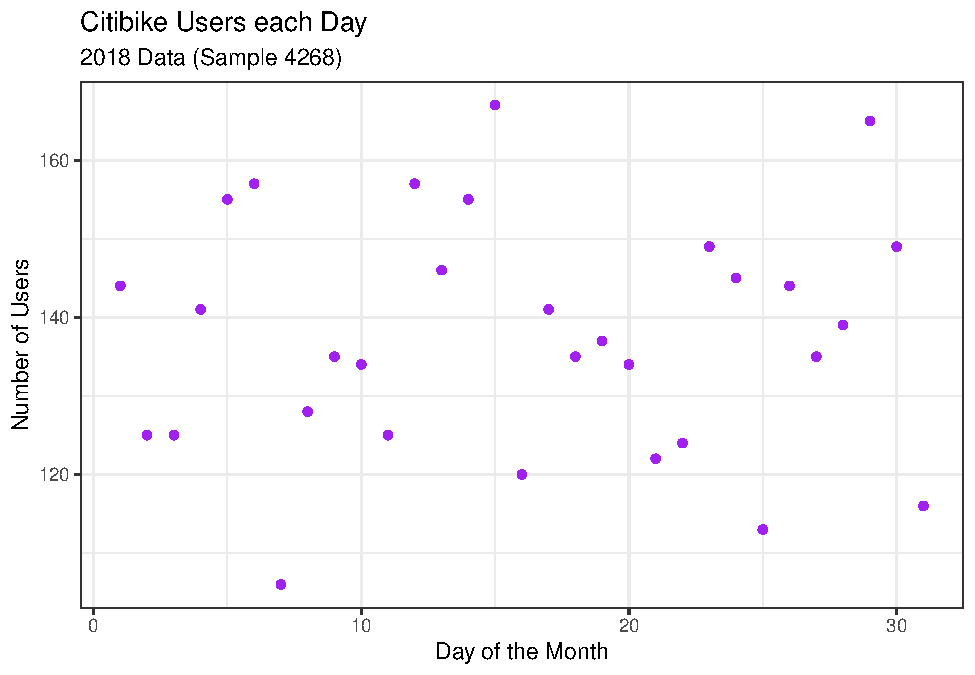
\includegraphics{nyc_bikes_presentation_janehogg_files/figure-latex/unnamed-chunk-14-1.pdf}
overall there is limited evidence of any trends in this data.

\begin{Shaded}
\begin{Highlighting}[]
\NormalTok{nyc\_bikes\_df }\SpecialCharTok{\%\textgreater{}\%}
  \FunctionTok{group\_by}\NormalTok{(day, gender) }\SpecialCharTok{\%\textgreater{}\%}
  \FunctionTok{count}\NormalTok{() }\SpecialCharTok{\%\textgreater{}\%}
  \FunctionTok{summarise}\NormalTok{(n) }\SpecialCharTok{\%\textgreater{}\%}
  \FunctionTok{ggplot}\NormalTok{(}\FunctionTok{aes}\NormalTok{(}\AttributeTok{x=}\NormalTok{ day, }\AttributeTok{y =}\NormalTok{ n, }\AttributeTok{group =}\NormalTok{ gender))}\SpecialCharTok{+}
  \FunctionTok{geom\_line}\NormalTok{(}\AttributeTok{colour =} \StringTok{"purple"}\NormalTok{)}\SpecialCharTok{+}
  \FunctionTok{theme\_bw}\NormalTok{()}\SpecialCharTok{+}
\FunctionTok{facet\_wrap}\NormalTok{(}\SpecialCharTok{\textasciitilde{}}\NormalTok{gender)}\SpecialCharTok{+}
  \FunctionTok{labs}\NormalTok{(}
    \AttributeTok{x =} \StringTok{" Day of the Month "}\NormalTok{,}
    \AttributeTok{y =} \StringTok{"Number of Users"}\NormalTok{,}
    \AttributeTok{title =} \StringTok{"Variation in Use v Gender"}\NormalTok{,}
    \AttributeTok{subtitle =} \StringTok{"2018 Data (Sample 4268)"}\NormalTok{,)}
\end{Highlighting}
\end{Shaded}

\begin{verbatim}
## `summarise()` has grouped output by 'day'. You can override using the `.groups`
## argument.
\end{verbatim}

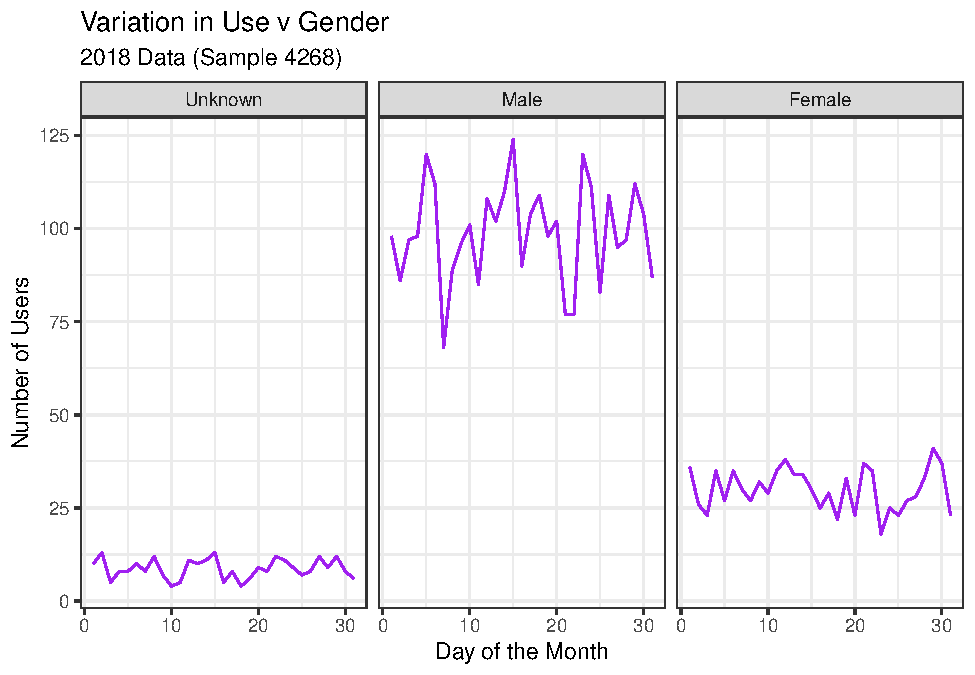
\includegraphics{nyc_bikes_presentation_janehogg_files/figure-latex/unnamed-chunk-15-1.pdf}

\end{document}
